\subsection{Introduction}

SHADOW is a ray-tracing program specially optimized for the design of x-ray optical systems in general and synchrotron radiation beamlines in particular.

SHADOW has demonstrated its reliability during four decades of utilization, supporting beamline design and optimization in most synchrotron facilities from 2$^\text{nd}$ to 4$^\text{th}$ generations. It has been used and cited in hundreds of publications.

\paragraph{History}
SHADOW was created by Franco Cerrina \cite{cerrina1984shadow} in the early 80's. SHADOW1 (1984-1990), written in Fortran77,  was running in VAX-VMS mainframes, and was used not only for the design of monochromators of ``Aladdin", a 2$^\text{nd}$ generation source at the University of Wisconsin, but also at other synchrotrons. SHADOW2 (1990-2010) run in Unix workstation and was also ported to Windows. The ShadowVUI visual interface, available in the XOP environment \cite{xop1997} popularized the use of SHADOW in many facilities and helped in the beamline design at the newly ESRF, a first source of 3$^\text{rd}$ generation. SHADOW3 \cite{shadow3} was released after a refactoring of the Fortran code to be compatible with new standards of Fortran9x. A Python Application Program Interface (API) \cite{Canestrari2011} was introduced that allowed direct Python scripting and opened the door to new interfaces. Indeed, a quantum leap in user interfacing, that make much easier the beamline design with SHADOW3 was done in ShadowOUI \cite{ShadowOUI}. It put together the power of the SHADOW3 kernel with the beautiful and efficient workflows from ORANGE\footnote{{\tt https://orangedatamining.com/}} \cite{ORANGE}. Very soon the power of ShadowOUI was boosted with new tools, like the HYBRID method for correcting ray tracing for coherent beams \cite{Shi2014}, databases for surface error\footnote{\tt https://github.com/oasys-kit/DabamFiles}, preprocessors for different elements, loops for thermal load calculations \cite{RebuffiThermal2020}, and high d-spacing crystals \cite{Yu2022}. ShadowOUI was integrated in OASYS \cite{OASYS} a larger suite of programs dedicated to synchrotron applications also including tools for wave optics simulations, the natural complement of ray tracing when dealing with coherent beams.

Just recently a new version, SHADOW4 \cite{shadow4_sri2025}, features a new kernel and a new interface, prepared for new generation of synchrotron sources.
The SHADOW4 kernel is a fully object-oriented package named {\tt shadow4}\footnote{{\tt https://github.com/oasys-kit/shadow4}}, fully implemented in Python. It benefited of the experience and some libraries developed for OASYS.
SHADOW4 uses modern and standard software engineering concepts that will permit a larger community of developers to help with new resources, tutorials, and documents.
It is naturally interface in OASYS2. 



\paragraph{Philosophy}

SHADOW generates and traces a beam along the optical system. The beam is a collection of rays in a given point of the beamline which are stored in a memory array. The optical system is a collection of optical elements (o.e.) (mirrors, multilayers, slits, screens, etc.) placed in a sequential order. 

Each ray is an array of 18 variables or ``columns" (they are like a columns in an excel representation of the array of rays, where the row refer to the ray number).
Each variable of column has an special physical meaning. The first six defines the geometry: spatial coordinates (Columns 1,2,3 or x, y and z, respectively) and the direction of the ray (cols. 4,5,6, or x’,y’ and z’, respectively). The rest of the columns defines the history of the ray traversing the optical system (electric vector for s-polarization (cols. 7,8,9) and p-polarization (cols. 16-18), flag for lost ray (10), wavelength (11) etc.).
In addition to the 18 columns physically stored, there are many other ``columns" that are calculated from the native 18. For example, the ray intensity (column 23) is calculated from the electric field components (columns 7,8,9,16,27,18).

The source is the beam at the starting point. It is generated by SHADOW by sampling the spatial, angular, energy and other qualities of the synchrotron radiations sources (i.e., bending magnets, wigglers and undulators) into a finite number of rays, using a Monte Carlo method. At the source position the intensity of each ray (or better, its probability of observation) is set to 1. This intensity will decrease along the beamline because of the interaction of the ray with the optical elements. The source generated by SHADOW samples linearly the real source, which allows scaling the intensity with the number of photons. There are several kind of sources in SHADOW:
\begin{itemize}
    \item Grid sources:the rays are not created by Monte Carlo sampling, but just distributed in grids (in cartesian or polar coordinates, and in real or divergence spaces).
    \item Geometrical sources: the rays are distibuted randomly folowing different distributions either in space (point, rectangular, elliptical, Gaussian, etc.) and in directions of divergence space (collimated, uniform, Gaussian, etc.). Each ray has is monochromatic (it has a single well dephiced photon energy), but polychromatic or white sources can be created sampling the ray energies using the desired energy spectrum.
    \item Synchrotron sources: Bending Magnet \cite{S4bendingmagnets}, Wiggler and Undulator \cite{S4undulators} sources are magnetic structures used for creating synchtrotron radiation in storage rings. SHADOW has very specialised and performant models to simulate these synchrotron sources. 
\end{itemize}

SHADOW traces the source sequentially thought each individual optical element of the optical system. SHADOW solves the intercept of each ray at a given o.e., calculates the output direction and the decrease in intensity. This decrease is calculated for each ray using a physical model (i.e. Fresnel equations for mirrors, Dynamical Theory of the Diffraction for perfect crystals, etc.)

In SHADOW, the  calculation of the beam modified by a beamline element can be separated in two parts: 
\begin{enumerate}
    \item the ``geometrical" model
    \item the ``physical" model
\end{enumerate}

The first one deals with the positioning of the rays as it arrives and leaves the element, the intersection with the optical surface, and how the element modifies the directions (e.g. beam reflection by a mirror, or refraction by a lens). The ``physical" model deals with the changes of ray's electric fields (that carry out the intensity) due to the interaction with the element. 

The operations of the ``geometrical" model are grouped in class family {\tt S4OpticalSurface}), whose subclasses contain the traditional surfaces in SHADOW, namely,
\begin{itemize}
    \item {\tt S4Conic}, for conic surfaces (described by a second-degree polynomial), including planes, spheres, ellipsoids, hyperboloids, paraboloids and the corresponding cylindrical ones \cite{S4Conic}
    \item {\tt S4Toroid}, a toroid (4$^\text{th}$-degree equation)
    \item {\tt S4Mesh}, a generic surface numerically defined over a regular mesh. 
\end{itemize}

The calculation of the reflectivity or transmittivity of the beamline elements requires the computation of material parameters, typically the refraction indices, the photon-material cross sections, the structure factors for crystals, etc. This computation needs to access tabulated data for the materials, that are available in different ways:

\begin{enumerate}
    \item {\bf Pre-processors.} Traditionally SHADOW works by separating the access to these data from the main kernel code, using the ``pre-processor" concept. A pre-processor is a standalone code that will prepare a ``material" file for SHADOW. Three pre-processors are available in SHADOW, {\tt PreRefl} containg refraction indices thus used for absorbers, lenses and mirror reflectivity calculations, {\tt Bragg} containing the ingredients of the structure factors thus used by crystals, and {\tt MLayer} containg the materials, refraction indices and structure of a multilatered element, thus used for multilayers.
    The use of pre-processor file is preserved in SHADOW4. There are good reasons for that: i) compatibility with old versions and re-use of pre-processor files, ii) the SHADOW4 package may work in standalone mode without importing external libraries, and iii) the use of pre-processor file is faster than the direct access to data libraries and is advantageous for loops and scripts.
    Pre-processors files can be created with the appropriate OASYS widgets. 
    \item {\bf DABAX} stands for DAtaBAse for X-ray applications. It is a compilation of tables\footnote{\tt https://github.com/oasys-kit/DabaxFiles} for X-ray applications with a collection of python programs
    \footnote{\tt https://github.com/oasys-kit/dabax}
    to access and process these tables.
    \item {\bf XRAYLIB}\footnote{\tt https://github.com/tschoonj/xraylib} \cite{Schoonjans2011} is an open-source library that provides a collection of X-ray interaction data and functions for use in scientific computing. It gives researchers and developers easy programmatic access to atomic and nuclear data relevant to X-ray physics, including cross-sections, fluorescence yields, line energies, and more. It is fully integrated in SHADOW4 and OASYS2.
\end{enumerate}


The advantages of DABAX is the decoupling of data from calculations — you can easily change the files in the database without needing to change the programs. OASYS widgets include menus that allows the user to choose their preferred data file. The need for fast access and data simplification for X-ray fluorescence applications drove the development of xraylib as a completely new tool — an ANSI C library providing convenient access to a large number of X-ray related databases, with a focus on quantitative X-ray fluorescence applications. The two libraries are complementary: DABAX is a flexible, file-based database system, while xraylib is a more streamlined programmatic library optimized for work that need high speed.

A powerful feature of the OASYS interface to SHADOW4 is the automatic generation of scripts. Every SHADOW4 widget has a ``tab" that displays the python script that runs the system. It can be exported and run outside the OASYS environment. It provides to the users the flexibility to customize and tailor calculations to their specifications, as well of performing scans of variables (e.g. for calculating tolerancies) or perform simulations with millions of rays to improve statistics and to compute errors in the parameters. 

\begin{figure}[H]
\label{fig:S4_reference_frame}
    \centering
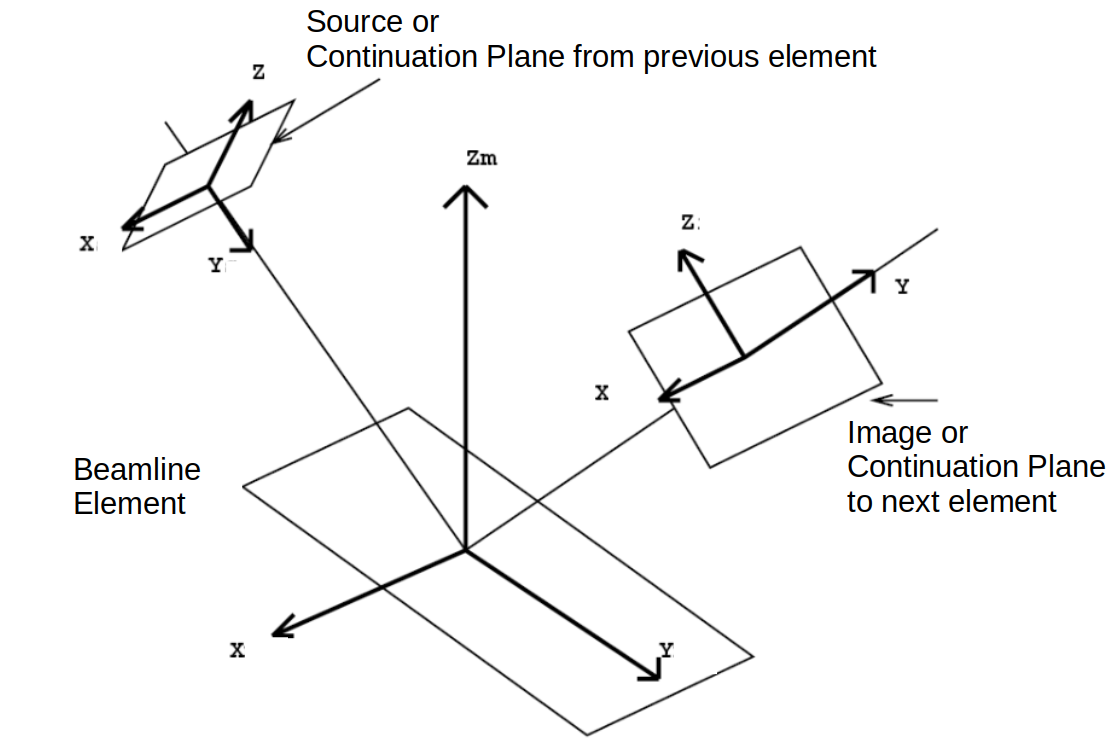
\includegraphics[width=0.9\linewidth]{reference-frames/S4_reference_frame.png}
\caption{SHADOW4 reference frame definitions: Source, beamline element, and image coordinates.}  
\end{figure}

